\documentclass[12pt]{article}
\usepackage{polski}
\usepackage[utf8]{inputenc}
\usepackage[T1]{fontenc}
\usepackage{times}

\usepackage{amsfonts}
\usepackage{amsmath}
\usepackage{bm}
\usepackage{mathtools}
\mathtoolsset{showonlyrefs}


\usepackage{tabularx}
\usepackage{array}
\newcolumntype{Y}{>{\centering\arraybackslash}X}
\newcolumntype{Z}{>{\centering\arraybackslash}p}
\usepackage{multirow}
\usepackage{hyperref}

\usepackage{enumitem}
\usepackage{float}


\usepackage{graphicx}
\usepackage{rotating}
\usepackage{subcaption}


%\usepackage{animate}

\renewcommand{\thesection}{\arabic{section}}
\renewcommand{\thesubsection}{\arabic{section}.\arabic{subsection}}
\usepackage{wrapfig}



\usepackage{amsmath}
\usepackage{amsthm}
\usepackage{dsfont}
\newtheorem{lema}{Lemma}

\newtheoremstyle{exer}{20pt}{10pt}{}{0pt}{\bfseries}{.\\}{.5em}{}
\theoremstyle{exer}
\newtheorem{ex}{Ex}

%\usepackage[a4paper,total={6in,10in}]{geometry}
\usepackage[a4paper,total={7in,10in}]{geometry}
%\newtheoremstyle{style name}{space above}{space below}{body font}{indent amount}{head font}{head punct}{after head space}{head spec}


\begin{document}
	\begin{titlepage}
		\begin{center}
			
			\textbf{\Huge  Analiza danych rzeczywistych przy pomocy modelu ARMA}
			
			\vspace{0.5cm}
			
			\vspace{1.5cm}
			
			\textbf{\LARGE Autorzy}\\
			\vspace{0.5cm}
			\large Kacper Budnik, 262286\\
			\large Maciej Karczewski, 262282\\
			
			
			\vfill
			
			\vspace{0.4cm}
			

			
			\vspace{0.8cm}
			Wydział Matematyki	
			\today
		\end{center}
	\end{titlepage}
	\tableofcontents
	\newpage
	
	\section{Wprowadzenie}
	
	\section{Przygotowanie danych do analizy}
	
	
	\section{Dekompozycja szeregu czasowego}
	\subsection{Wykresy dla surowych danych}
	
	\subsection{Transformacja Boxa-Coxa}

	\subsection{Różnicowanie sezonowe}
	
	
	
	\section{Ocena dopasowania modelu}
	W celu oceny dopasowania modelu do danych zobaczymy jak wyglądają przedziały ufności na poziomie $\alpha = 5\%$ dla ACF i PACF 
	\begin{figure}[H]
		\centering
		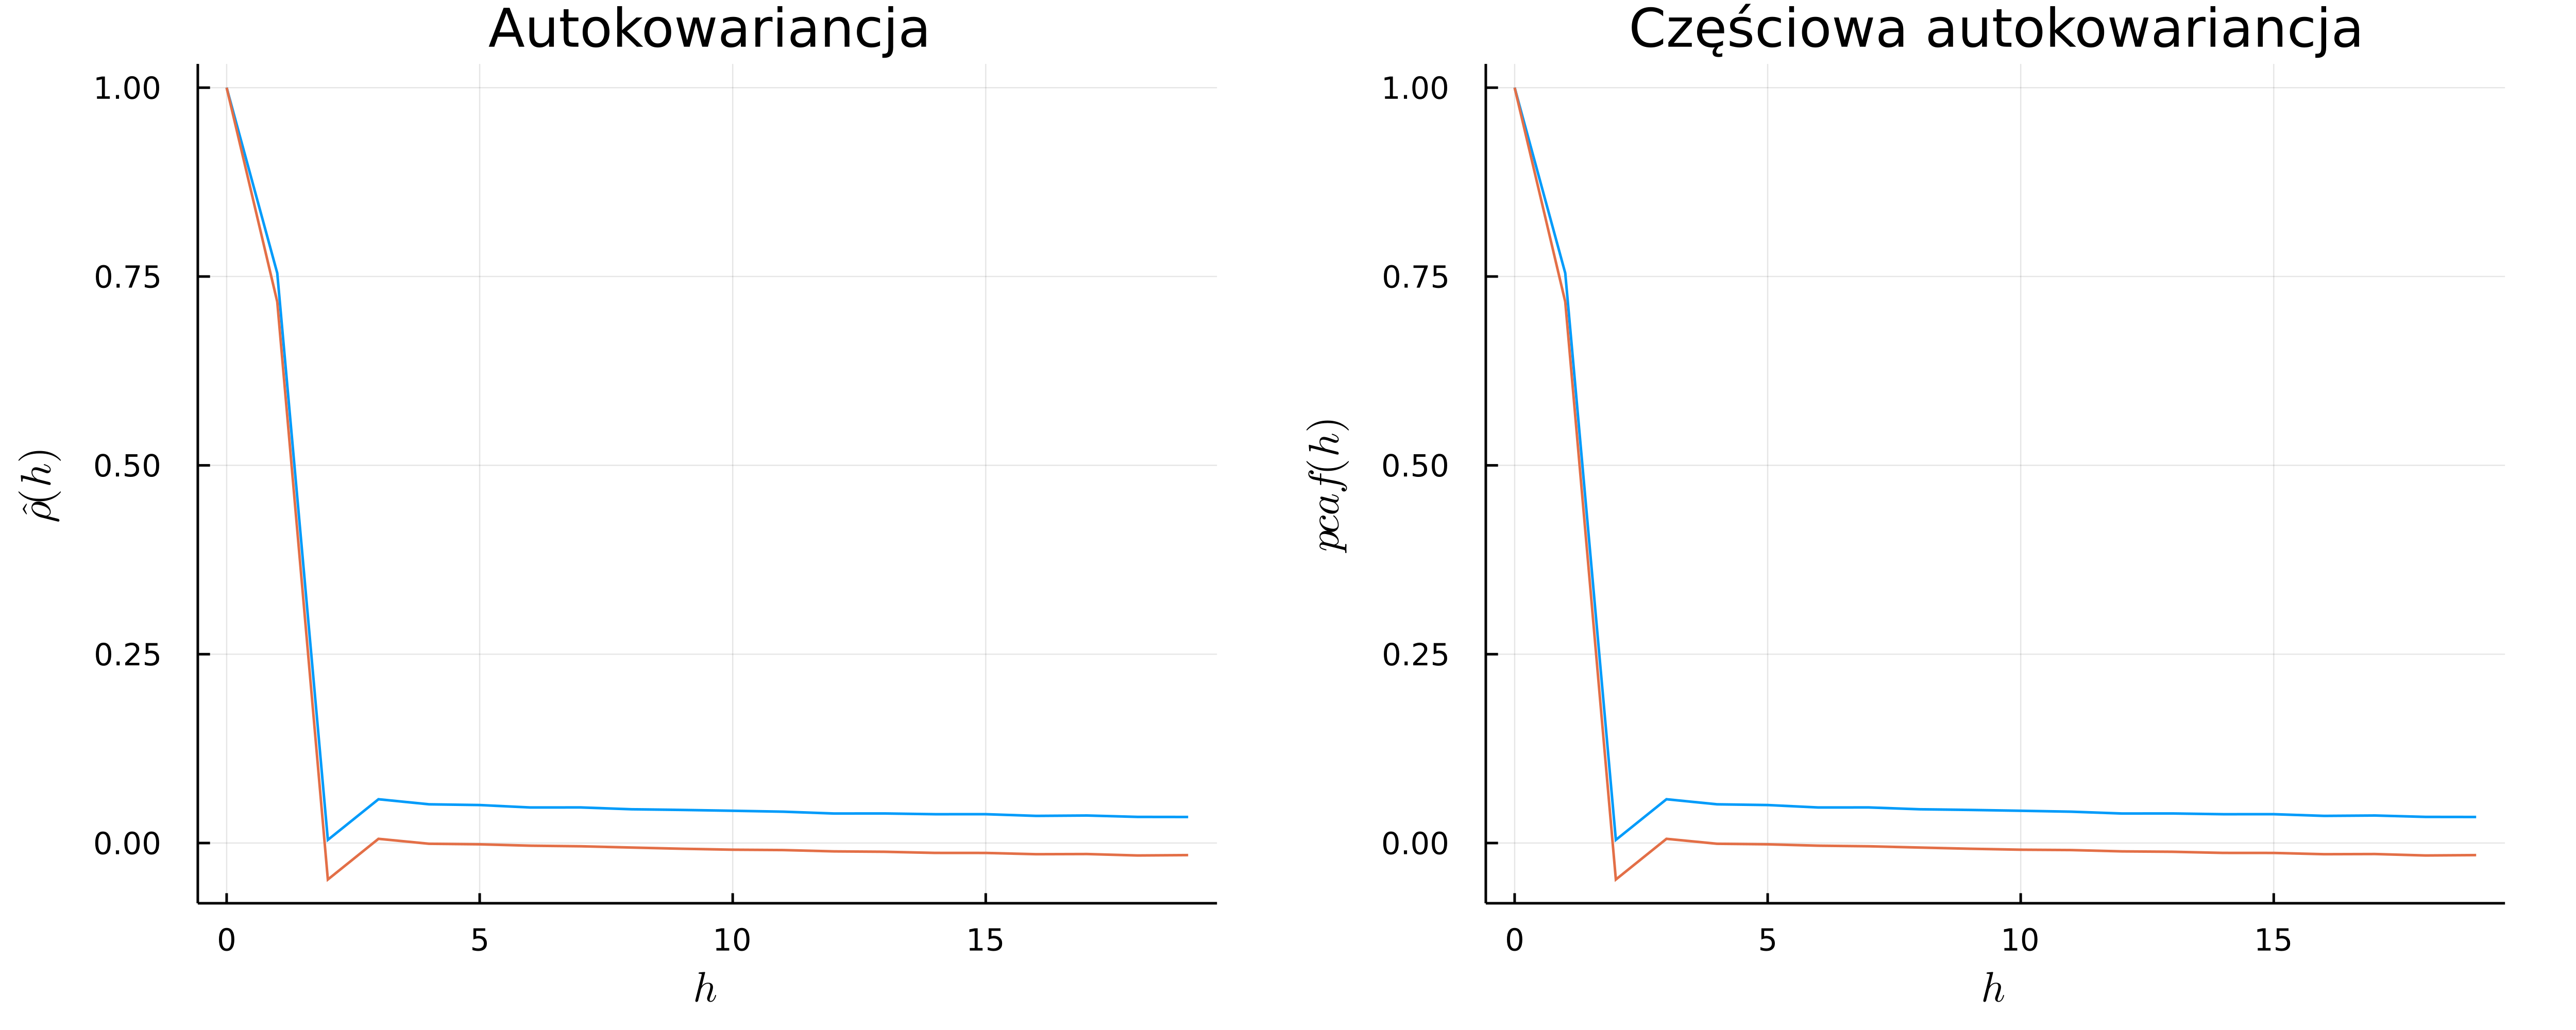
\includegraphics[width=3\columnwidth/4]{img/acf_pacf.png}
		\caption{Przedziały ufności dla ACF i PACF dla naszego modelu}
		\label{fig:model_acf_pacf}
	\end{figure}
	Jak możemy zobaczyć na wykresie \ref{fig:model_acf_pacf} istnieje tylko okresowa zależność pomiędzy danymi w modelu.
	
	
	Następnie porównamy trajektorię z liniami kwantylowymi dla naszego modelu
	\begin{figure}[H]
		\centering
		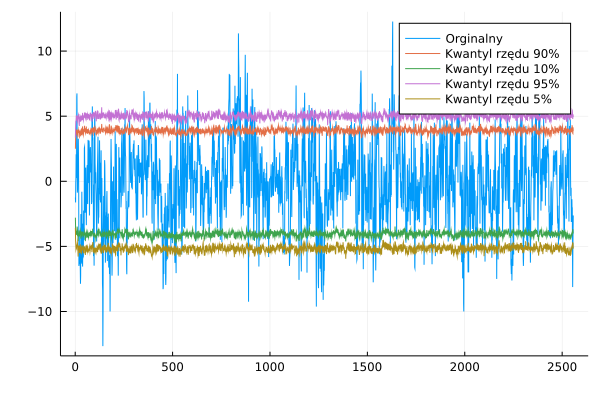
\includegraphics[width=3\columnwidth/4]{img/linie_kwantylowe.png}
		\caption{Porównanie orginalnych danych z liniami kwantylowymi modelu}
		\label{fig:linie_kwantylowe}
	\end{figure}
Analizując linie kwantylowe naszego modelu  pokazane na wykresie \ref{fig:linie_kwantylowe} możemy zauważyć, że model w miarę dobrze się sprawdza dla naszych danych. 


Patrząc na wykres zależności w modelu \ref{fig:model_acf_pacf} oraz na wykres z liniamy kwantylowymi \ref{fig:linie_kwantylowe} dochodzimy do wniosku, że model dobrze się sprawdza dla naszych danych.


	\section{Analiza szumu}
	Podczas tworzenia modelu ARMA zakładaliśmy następujące warunki odnośnie szumu
	\begin{enumerate}
		\item $\mathbb{E}\xi_i=0$ $\forall i$ ,
		\item $Var\xi_i=\sigma^2<\infty\quad\forall i$,
		\item $\xi_i\perp\!\!\!\perp\xi_j$ dla $i\neq j$,
	\end{enumerate}
	
	\subsection{Stała średnia równa 0}
	Sprawdzimy czy rezidua naszego modelu mają stałą średnią równą $0$. W tym celu zobaczymy jak wyglądają nasze wartości resztowe.
	
	\begin{figure}[H]
	\centering
	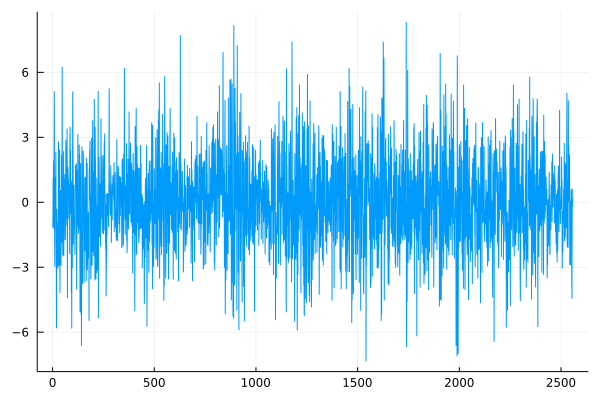
\includegraphics[width=3\columnwidth/4]{img/residua.png}
	\caption{Residua naszego modelu}
	\label{fig:residua}
\end{figure}
 Jak możemy zobaczyć na \ref{fig:residua} średnia jest stała w czasie i wynosi w przybliżeniu $0$. 
 W celu upewnienia się wykonamy też t test dla jednej zmiennej.
 	\begin{figure}[H]
 	\centering
 	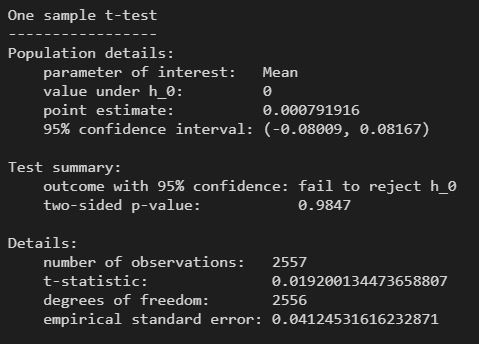
\includegraphics[width=3\columnwidth/4]{img/t_test.png}
 	\caption{Test t dla naszych wartości resztowych}
 	\label{t_test}
 \end{figure}
Jak możemy zobaczyć test t \ref{t_test} nie miał podstaw do odrzucenia hipotezy zerowej, która mówiła ,że średnia wynosi $0$. Test zwrócił $p$-value równe $0.9847$.
Tak więc możemy przyjąć, że średnia jest stała i równa $0$

\subsection{Stała wariancja}
Z wykresu \ref{fig:residua} możemy odczytać, że wariancja jest stała.Dodatkowo możemy obliczyć ,że  należy ona do przedziału $[4.141 ; 4.554]$ na poziomie ufności $\alpha = 5\%$

\subsection{Niezależność szumu}
Sprawdzimy teraz założenie dotyczące niezależności szumu w czasie. Sprawdzimy na początek wykres autokowariancji i częściowej autokowariancji. 
\begin{figure}[H]
	\centering
	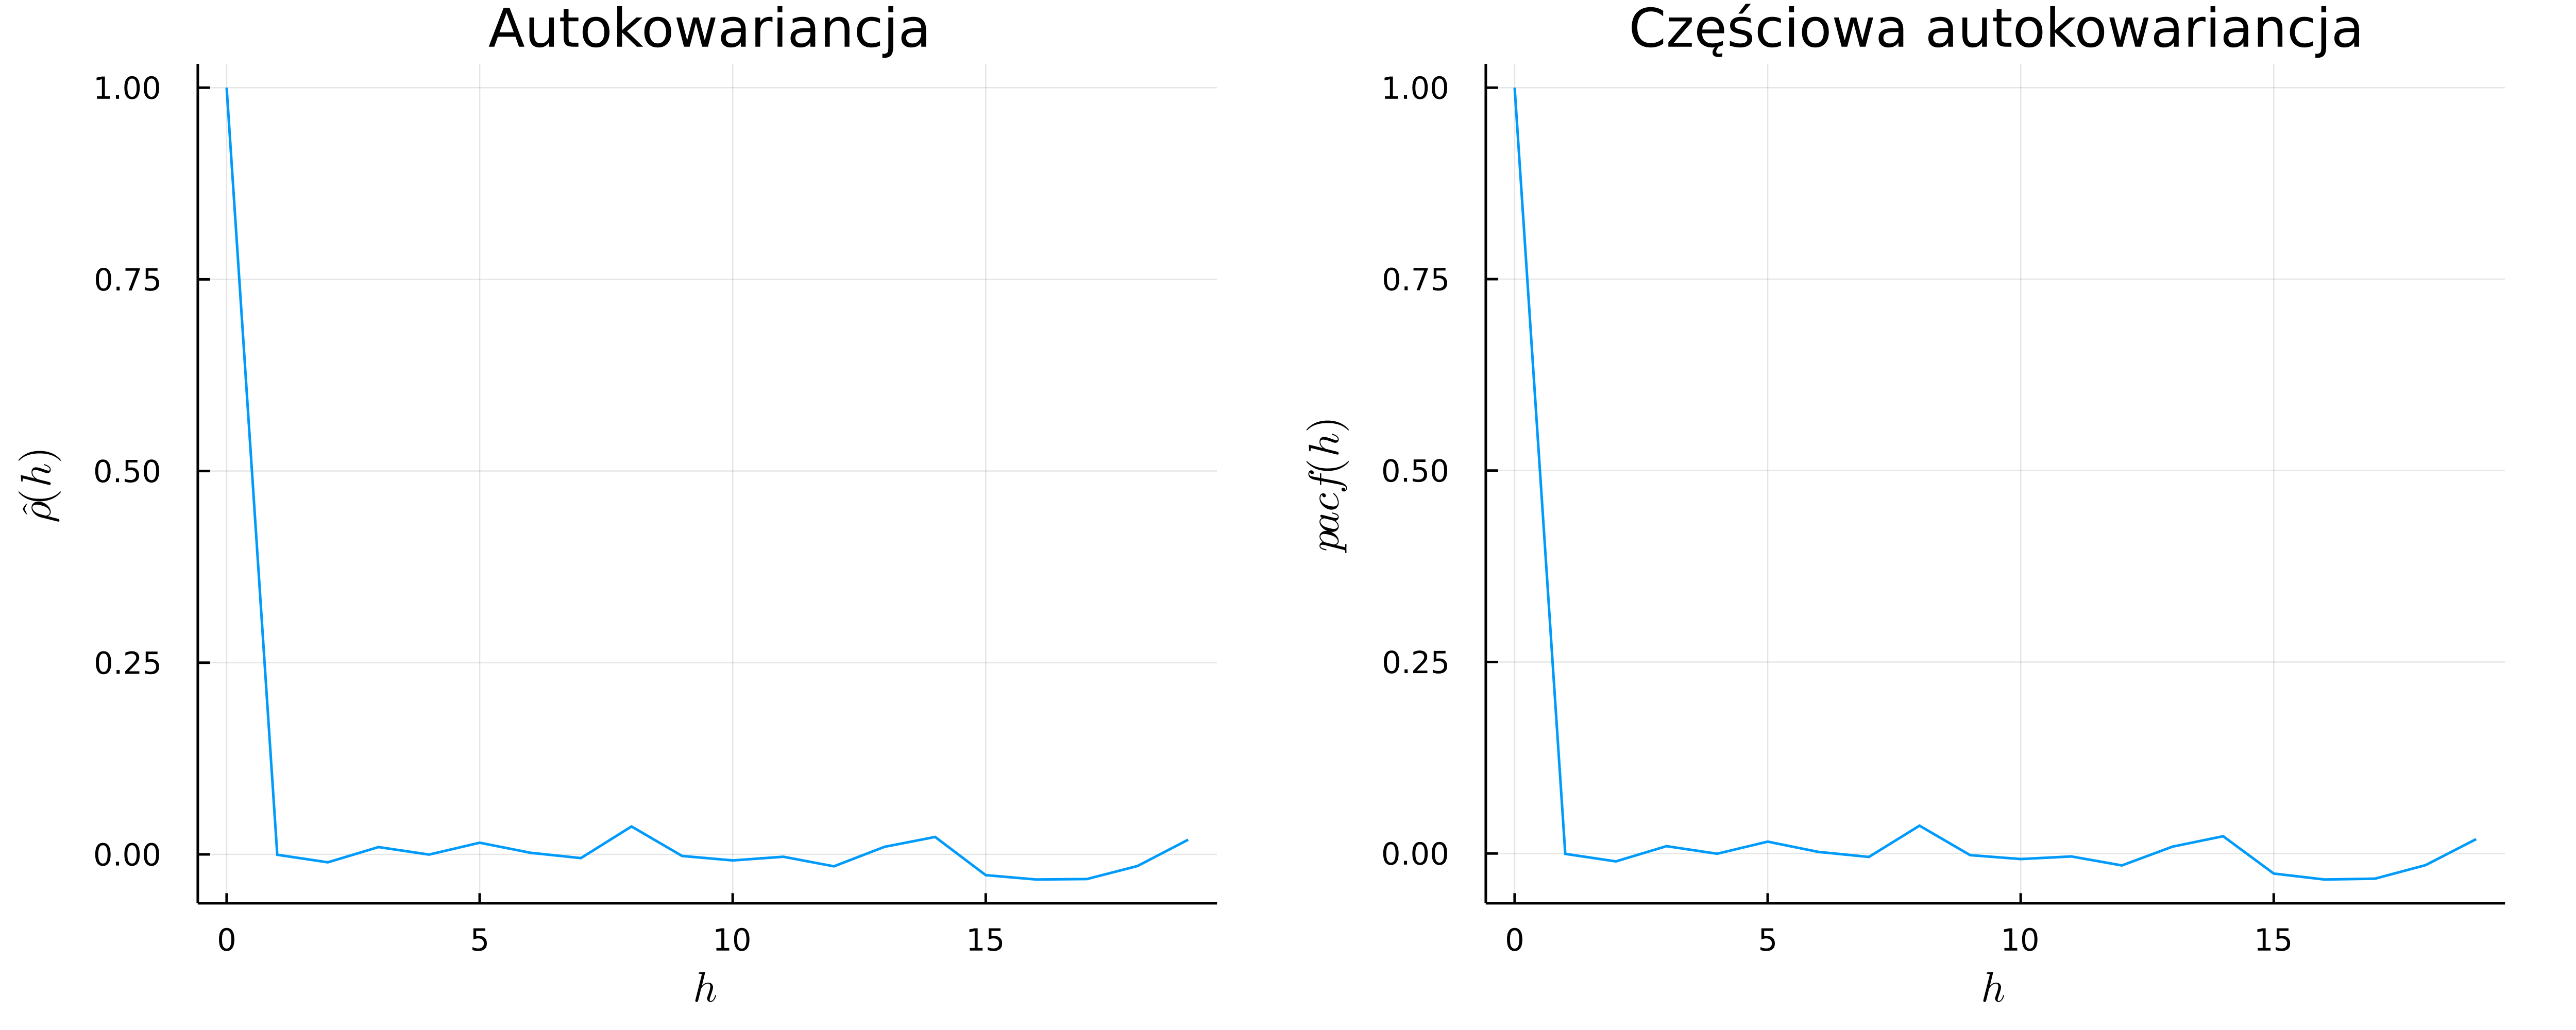
\includegraphics[width=3\columnwidth/4]{img/acf_pacf_residua.png}
	\caption{ACF i PACF dla wartości resztkowych modelu}
	\label{fig:residua_acf_pacf}
\end{figure}
Na wykresie \ref{fig:residua_acf_pacf} możemy  zobaczyć że mamy szum jest zależny tylko od siebie w tym samym momencie.

Dodatkowo wykonamy test Ljunga-Boxa by upewnić się że szum jest niezależny od siebie.
\begin{figure}[H]
	\centering
	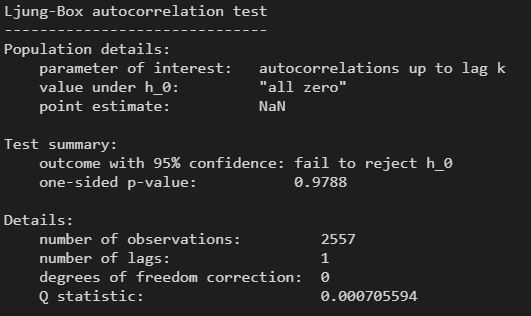
\includegraphics[width=3\columnwidth/4]{img/Ljung-Box.png}
	\caption{Test Ljunga Boxa dla naszych wartości resztowych}
	\label{Test Ljunga Boxa}
\end{figure}

Test nam potwierdza, że nie mamy podstaw do odrzucenia hipotezy mówiącej, że szum jest niezależny od siebie.

\subsection{Założenie o normalności rozkładu}
Sprawdzimy teraz dodatkowe założenie mówiące o tym że szum ma rozkład normalny.
Na początku sprawdzimy histogram wraz z gęstością empiryczną i teoretyczną rozkładu normalnego.
\begin{figure}[H]
	\centering
	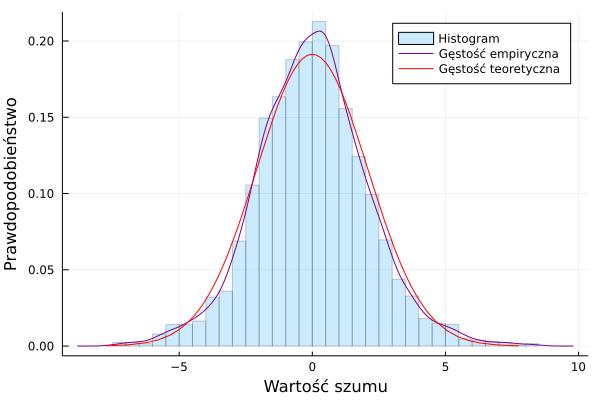
\includegraphics[width=3\columnwidth/4]{img/density.png}
	\caption{Histogram, gęstość rozkładu szumu wraz z rozkładem normalnym}
	\label{fig:density}
\end{figure}

Patrząc na histogram wraz z gęstościami \ref{fig:density} możemy załuważyć, że rozkład wartości resztowych może być normalny ale nie musi. W celu dalszego sprawdzenia normalności zobaczymy jak będzie wyglądał wykres kwantylowy.

\begin{figure}[H]
	\centering
	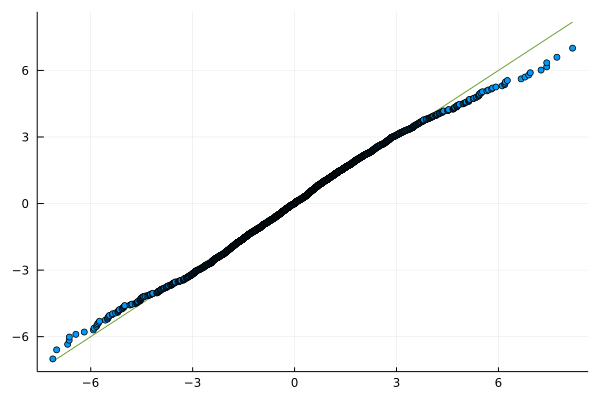
\includegraphics[width=3\columnwidth/4]{img/qqplot.png}
	\caption{Qqplot dla wartości resztowych}
	\label{fig:qqplot}
\end{figure}

Analizując wykres kwantylowy \ref{fig:qqplot} widzimy, że potencjalnie ogony rozkładu niezf=gadzają się z rozkładem normalnym. W celu ostatecznej weryfikacji normalności wykonamy test Andersona Darlinga. 
\begin{figure}[H]
	\centering
	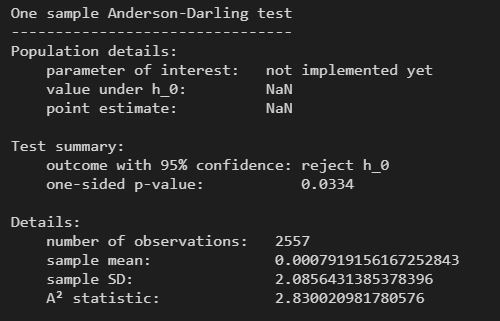
\includegraphics[width=3\columnwidth/4]{img/ad_test.png}
	\caption{Test Andersona Darlinga dla naszych wartości resztowych}
	\label{Test_AD}
\end{figure}
Test Andersona Darlinga \ref{Test_AD} odrzuca hipotezę o normalności rozkładu. Dla naszych danych $p$-value wynosi $3.3\%$. 

Podsumowując rozkład szumu nie ma rozkładu normalnego.
	\section{Wnioski autorów}
	
	
\end{document}